\documentclass[12pt]{report}
% éèàçù (pour que le 'charset' soit détecté automatiquement par l'éditeur de texte)

\usepackage[utf8x]{inputenc}
\usepackage[T1]{fontenc}
\usepackage{hyperref}
\usepackage[english]{babel}
%\usepackage[dvips]{graphicx}
\usepackage{graphicx}
\usepackage{tocloft} % personalisation de la table des matières (pour avoir "TP #" sans problème d'espacement)
\usepackage{bbm} %pour avoir Q
\usepackage{slashbox}
\usepackage{lmodern} % amélioration des polices ?


\usepackage{fullpage} % pour avoir des pages pleines

\newtheorem{iter}{}
\newtheorem{version}{Version}
\newtheorem{question}{Question}[chapter]

\newcommand{\code}[1]{\texttt{#1}}
\newcommand{\dom}{\string:\string:}
\newcommand{\exo}[1]{\textit{#1}}
\newcommand{\eclipse}{ECLiPSe}
\newcommand{\prolog}{Prolog}

\graphicspath{{figures/}} % dossier où trouver les fichiers de \includegraphics


\title{
\begin{flushleft}
{
\includegraphics[width=4cm]{insa.pdf}}
\vspace{-2cm}
\end{flushleft}
\begin{flushright}
\normalsize
Year 2014--2015
\end{flushright}
\vspace{10ex}
\rule{12cm}{1mm}
\huge{\\Constraint programming}\\
\vspace{5ex}
\Large{Practical work handbook}\\
\vspace{5ex}
\large{\it Mireille Ducassé : mireille.ducasse@insa-rennes.fr\\
%Haykel Boukadida : haykel.boukadida@yahoo.fr\\
%Aymeric Hervieu : aymeric.hervieu@irisa.fr
José Ángel Galindo Duarte : jagalindo@us.es\\
Pascal Garcia : Pascal.Garcia@insa-rennes.fr
}\\
\rule{12cm}{1mm}
\vspace{15ex}
\begin{flushleft}
\begin{tabular}{l}
\textit{4th year}\\
\textit{Informatics departement}\\
\textit{INSA Rennes}
\end{tabular}
\end{flushleft}
}
\author{}
\date{}

\setcounter{tocdepth}{0}

\begin{document}

\pagestyle{empty}
\maketitle
%\newpage
\pagestyle{plain}
\renewcommand{\chaptername}{TP} % On met l'intitulé 'nom de chapitre' à TP 
\renewcommand{\thechapter}{\arabic{chapter}}
%\renewcommand{\thefigure}{\arabic{chapter}.\arabic{figure}}
\renewcommand{\thesection}{\arabic{section}}
\renewcommand{\thesubsection}{\thesection.\arabic{subsection}}

{
\setlength{\baselineskip}{1.8\baselineskip} % On change temporairement l'interligne pour la table des matières
%\cftsetindents{chapter}{0pt}{1.3cm} 
%\renewcommand{\contentsname}{\pagebreak\centerline{Sommaire}} % Comme
%il est au début c'est un Sommaire.
\renewcommand{\contentsname}{\centerline{Sommaire}} % Comme il est au début c'est un Sommaire.
\tableofcontents
}

\cleardoublepage
\chapter*{Foreword}

This workbook to present various concrete problems
combinatorial research and optimization. The purpose of this lab is to
teach you how to model these problems by using programming
by constraints. A strong point of constraint programming is
the resolution of a problem is independent of its modeling and
that, therefore, we can use this type of programming without
know the underlying resolution algorithms (propagation,
branch and bound, \ ldots). However, you will quickly
has an understanding of these algorithms is needed to
understand what is happening and, more concretely, debug your
programs.



\section*{Thanks}

Ce cahier de TP a été initialement conçu par Edouard Monnier avec
l'aide de Christiane Hespel. Il a été ensuite régulièrement remanié
par les intervenants successifs, en particulier, Matthieu Carlier,
Florence Charreteur, Tristan Denmat, Coralie Haese, Vincent Montfort,
Harold Mouchère, Matthieu Petit et Benoit Ronflette.

\addcontentsline{toc}{chapter}{Introduction à ECLiPSe \prolog}
\chapter*{Introduction à ECLiPSe \prolog}

Tous les TP, sauf celui du chapitre~\ref{chapitre:choco}, seront faits
en ECLiPSe\footnote{ECLiPSe est téléchargeable gratuitement depuis le
  site du projet : \url{http://eclipseclp.org}}. Un prérequis est donc
d'être à l'aise avec \prolog, notamment avec les algorithmes
d'\textbf{unification} et de \textbf{backtracking} (cf chapitre 2 du
cours).  Vous pourrez utiliser deux extensions de \prolog: les
tableaux et les itérateurs (présentés dans la suite, ainsi que dans
l'annexe du cours). \prolog{} permet de résoudre des contraintes
portant sur des arbres (= des termes \prolog) mais c'est insuffisant
dès lors que les problèmes à résoudre sont numériques ou que les
contraintes entre variables sont complexes. Dans ce cas nous
utiliserons deux librairies d'ECLiPSe :
\begin{itemize}
\item \emph{ic} pour résoudre des problèmes numériques où les
  variables sont des entiers bornés.
\item \emph{ic\_symbolic} pour résoudre des problèmes où les variables
  sont de type énuméré, c'est à dire que leur valeur appartient à un
  ensemble de valeurs symboliques, par exemple $\left\lbrace thé,
    café, eau, lait, jus\right\rbrace$ (cf. TP~\ref{tp2}).\\
\end{itemize} 

Sur les machines de l'INSA, ECLiPSe se lance à l'aide de la commande
\texttt{eclipsep}. Voici un exemple de début de session :

\begin{verbatim}
$ eclipsep
ECLiPSe Constraint Logic Programming System [kernel]
...
Version 6.0 #162 (i386_linux), Mon Sep 20 06:09 2010
[eclipse 1]:
\end{verbatim}

Les fichiers ECLiPSe portent l'extension \texttt{ecl} (ou  \texttt{pl}).
Un fichier \texttt{tp1.ecl} se charge dans l'environnement avec \og
\texttt{[tp1].} {\fg} (commande standard des environnements
\prolog). Attention à ne pas mettre de majuscule en début de nom de
fichier car dans ce cas \prolog{} croirait que c'est le nom d'une
variable.

\section{Les tableaux}
En ECLiPSe, la structure de données \textit{tableau} existe. Vous
pouvez l'utiliser à la place de listes lorsque vous avez besoin de
faire des accès directs aux éléments d'une liste ou pour définir des
structures de données à plusieurs dimensions (ex : matrices $N \times
M$).

Un tableau est défini avec le foncteur \verb|[]/1|. De plus, le
prédicat \verb|dim/2| permet de lier un tableau à sa dimension. Ex:
\begin{verbatim}
[Eclipse 1]:  Tab_1 = [](1,2,3),
              dim(Tab_1,Dim). 

Tab_1 = [](1, 2, 3)
Dim = [3]

[Eclipse 2]:  Tab_2 = []([](1,2,3),[](4,5,6)),
              dim(Tab_2,Dim). 

Tab_2 = []([](1,2,3),[](4,5,6))
Dim = [2,3]

[Eclipse 3]: dim(Tab,[3,3]).

Tab = []([](_183, _184, _185), [](_179, _180, _181), [](_175, _176, _177))
\end{verbatim}
N.B : dans le dernier exemple, le fait d'utiliser une variable non instanciée comme premier paramètre de \verb|dim| entraîne la création d'un tableau de dimension $3 \times 3$ ne contenant que des variables.


L'accès aux éléments d'un tableau se fait via le prédicat
\verb|is/2|. {\bf Vous ne pouvez pas utiliser l'unification directement.} Ex:
\begin{verbatim}
[Eclipse 4]: Tab_1 = [](1, 2, 3),
             Var = Tab_1[2].

Var = [](1, 2, 3)[2]

[Eclipse 5]: Tab_1 = [](1, 2, 3),
             Var is Tab_1[2].

Var = 2

[Eclipse 6]: Tab_2 = []([](1, 2, 3),[](4, 5, 6)), 
             Var is Tab_2[1,3].

Var = 3.
\end{verbatim}
Néanmoins, vous pouvez utiliser T[i] dans des expressions de \emph{ic}:
\begin{verbatim}
[Eclipse 7]: Tab_1 = [](1, 2, 3),
             Tab_1[2] + Tab_1[3] #= Var

Var = 5.
\end{verbatim}


\section{Les itérateurs}
ECLiPSe permet l'utilisation d'itérateurs pour introduire du contrôle
dans \prolog. Ces itérateurs ne sont que du sucre syntaxique qui est
transformé en \prolog{} pur à la compilation (cf chapitre du cours
portant sur la préparation des TPs). Il faut garder cela en tête, par
exemple les erreurs de compilation font référence aux lignes du
programme transformé et non pas du programme initial. D'autre part,
\eclipse{} trace le programme transformé.

La forme générale est
\begin{verbatim}
(Itérateur1, ..., ItérateurN do Actions)
\end{verbatim}
A chaque itération (ou chaque ``tour de boucle''), les itérateurs de 1
à n évoluent d'un pas et à chaque pas les prédicats de \verb|Actions|
sont appelés. Attention, cela ne correspond pas à des itérations
imbriquées. Par contre, vous pouvez faire des imbrications en
utilisant des itérateurs dans \verb|Actions|.

Il existe trois itérateurs principaux.

%\begin{iter} Pour tout élément de : \verb|foreach(Elem,List)|
\subsection{Pour tout élément de : {\tt foreach(Elem,List)}}
% \\
  A l'itération $i$, la variable logique $Elem$ est unifiée au i\up{ème}
  élément de la liste $List$. \textbf{Attention, la variable $Elem$ est locale à l'itérateur}. Ex: 
\begin{verbatim}
:- ( foreach(Elem,[1, 2, 3]) 
   do 
     write(Elem)
   ).

123

:- ( foreach(Elem, [1, 2, 3]), 
     foreach(Elem2, List) 
   do 
     Elem2 is Elem + 5
   ). 

List = [6, 7, 8]
\end{verbatim}

%\end{iter}
 
%\begin{iter} Pour tout entier entre : \verb|for(Indice,Min,Max)| \\
\subsection{Pour tout entier entre : {\tt for(Indice,Min,Max)}}
  \verb!for! est une spécialisation de \verb!foreach! pour les variables
  entières. Elle fait varier la variable $Indice$ de $Min$ à $Max$ en passant par
  tous les entiers. Ex: 
\begin{verbatim}
:- ( for(Indice, 1, 3) 
   do 
      write(Indice)
   ).

123
\end{verbatim}
%\end{iter}

 
%\begin{iter} Accumulateur : \verb|fromto(Debut,In,Out,Fin)| \\
\subsection{Accumulateur : {\tt fromto(Debut,In,Out,Fin)}}
  fromto est un accumulateur dont la
  valeur initiale est \verb|Debut|, la valeur courante d'entrée est
  \verb|In|, la valeur courante de sortie est \verb|Out| et la valeur
  finale est \verb|Fin|. Le calcul permettant de passer de Out à In
  doit être explicité dans les prédicats \verb|Actions| associés au
  fromto. Au premier pas d'itération, \verb|In| vaut \verb|Debut|, au
  pas $i$ $\verb|In|_i$ vaut $\verb|Out|_{i - 1}$, au dernier
  pas \verb|Out| vaut \verb|Fin|. Ex: 
\begin{verbatim}
:- ( fromto(1, In, Out, 3) 
   do 
      Out is In + 1, 
      write(In)
   ).

123  
\end{verbatim}

fromto est souvent utilisé avec un autre itérateur. L'exemple suivant illustre la puissance du fromto :
\begin{verbatim}
inverse(List,LInverse):- 
    ( foreach(Elem, List), 
      fromto([], In, Out, LInverse) 
    do 
       Out = [Elem | In]
    ).

:- inverse([1, 2, 3], List).

List = [3, 2, 1]
\end{verbatim}
%\end{iter}

\subsection*{Portée des itérateurs}
Comme détaillé dans l'annexe du cours, les variables utilisées dans la
partie $Actions$ d'un itérateur et ne figurant pas dans les paramètres
de l'itérateur sont considérées comme locales à cet itérateur.  Par
exemple, le prédicat suivant ne fonctionnera pas~:
\begin{verbatim}
afficheKO(Tab):-
    dim(Tab, [Dim]),
    ( for(Indice, 1, Dim),
    do 
      Var is Tab[Indice],
      write(Var)
    ).
\end{verbatim}
En effet, l'appel \verb|Var is Tab[Indice]| échouera car \verb|Tab| est considérée comme étant une variable locale et n'est donc pas instancée. 

Afin de faire passer une variable du programme dans la portée d'un itérateur, il faut déclarer explicitement que cette variable est utilisée par l'itérateur via le prédicat
 \verb|param| (d'arité variable).\\
Ex: 
\begin{verbatim}
afficheOK(Tab) :-
    dim(Tab, [Dim]),    
    ( for(Indice, 1, Dim), 
      param(Tab) 
    do 
       Var is Tab[Indice], 
       write(Var)
    ). 
\end{verbatim}

\section{Les domaines finis}

Comme détaillé en cours, un problème de contraintes à domaines finis
est constitué d'un ensemble de contraintes portant sur des variables
et d'un ensemble de domaines finis dans lesquels les variables peuvent
prendre leur valeur. Résoudre un tel problème vise à trouver une
instanciation des variables dans leur domaine respectif telle que
toutes les contraintes soient satisfaites. La résolution d'un problème
de contraintes à domaines finis est basée sur deux principes :

\begin{itemize}

\item la \textbf{propagation} de contraintes. Chaque contrainte est analysée
      séparément afin d'éliminer des valeurs de domaines qui ne peuvent pas
      faire partie d'une solution. Par exemple, si l'on considère la contrainte
      $X<Y$ avec les domaines $D_x = D_y = 0 .. 10$, l'algorithme de
      propagation d'ECLiPSe va réduire les domaines à $D_x = 0 .. 9$ et $D_y =
      1 .. 10$. Si l'on ajoute la contrainte $X>Y$, l'algorithme de propagation
      va déduire $D_x = 2 .. 9$ et $D_y = 1 .. 8$, puis réexaminer la première
      contrainte. Ainsi de suite jusqu'à ce que les domaines soient $D_x = D_y
      = \emptyset$.

\item l'\textbf{énumération}. Lorsque la propagation ne suffit pas à trouver
      une solution ou à montrer qu'il n'y en a pas, l'énumération est utilisée.
      Elle consiste à fixer arbitrairement une valeur à une variable. 

\end{itemize}

Notez bien que ces deux algorithmes sont appelés de nombreuses fois pendant la
résolution de contraintes. Une phase de propagation est effectuée, puis une
énumération, puis une phase de propagation prenant en compte l'énumération
effectuée, etc.\\

La requête de chargement de la bibliothèque des domaines finis
numériques est :
\begin{verbatim}
:- lib(ic).
\end{verbatim}

Les principales contraintes de \emph{ic} sont des contraintes numériques :
des équations (\code{\#=}), des inéquations (\code{\#<} , \code{\#>},
\code{\#=<}, \code{\#>=}), des diséquations (\code{\#$\backslash$=}) dont les
membres sont des termes comportant des variables à domaine fini.

Le domaine d'une variable entière est défini grâce au prédicat \code{\#\dom/2} :

\begin{itemize}
\item \code{V \#\dom{} D} contraint la variable $V$ à appartenir au domaine $D$ ;
\item \code{Lv \#\dom{} D} contraint chaque variable de la liste \verb|Lv|
  à appartenir au domaine $D$.
\end{itemize}

Le domaine $D$ est spécifié soit par la liste des valeurs qu'il contient, soit
par un intervalle $\mathit{min}..\mathit{max}$, etc. (voir documentation).\\

L'algorithme de propagation est lancé dès qu'une contrainte est posée
dans ECLiPSe. Par contre l'algorithme d'énumération doit être appelé
\textbf{explicitement} en utilisant les prédicats \code{labeling/1},
\code{search/6}, ou bien une version customisée de labeling (cf
chapitre 4 du cours).
%
\code{labeling(Lv)} réussit pour chaque assignation des variables de
$L_v$ à une valeur de leur domaine qui respecte les contraintes.\\

Il est possible de faire de l'optimisation dans les domaines finis en utilisant
un algorithme de \textbf{branch and bound}. Dans la bibliothèque
\code{branch\_and\_bound} de \emph{ic}, le prédicat \code{minimize(Pred,Var)} recherche une solution de
\verb|Pred| qui minimise la valeur de \verb|Var|.

\subsection*{Les domaines symboliques}

On appelle domaine symbolique un domaine constitué d'un ensemble fini
de valeurs non numérique.  Dans ce cas, le domaine d'une variable est
un ensemble fini de terminaux, par exemple~: \verb|Day &:: week|, avec
\verb|week| le domaine symbolique représentant l'ensemble fini \\
\verb|{mo, tu, we, th, fr, sa, su}|.

La requête de chargement de la bibliothèque des domaines symboliques est :
\begin{verbatim}
:- lib(ic_symbolic).
\end{verbatim}

On retrouve alors les mêmes opérateurs que ceux décrits pour les
domaines finis numériques à la différence que ceux-ci débutent par
\code{\&} au lieu de \code{\#}.

Pour définir un domaine \emph{couleur} de manière locale on peut
utiliser le prédicat :
\begin{verbatim}
:- local domain(couleur(rouge,vert,bleu)).
\end{verbatim}

Le domaine est défini par un prédicat dont le foncteur est le nom du
domaine et les arguments sont les atomes qui représentent les valeurs
possibles du domaine. L'arité du prédicat correspond donc à l'arité du
domaine (ici 3 couleurs).

% Ce type de domaine est ordonné et son ordre dépend de la structure de
% définition du domaine, les valeurs du domaine sont liées aux entiers
% naturels tel que le premier argument soit 1, le second 2, etc. La
% bibliothèque \emph{ic\_symbolic} utilise cet ordre de manière interne.

\section{Enumération :  \code{labeling} et \code{search}}
\label{intro:labeling}

Les deux prédicats \code{labeling} et \code{search} sont utilisés pour
pour guider l'énumération de valeurs possibles pour les variables
lorsque la propagation ne suffit pas pour trouver une solution.

Attention : comme vu en détail dans le chapitre 4 du cours, ces deux
prédicats ne couvrent pas toutes les manières de guider
l'énumération. Dans certains cas, ils ne sont pas suffisamment
efficaces. Dans le TP~\ref{sec:balancoire} vous devrez proposer des
stratégies d'énumération mieux adaptées au problème en customisant le
prédicat \code{labeling}.


\subsection{Labeling}
Le prédicat \code{labeling} choisit une variable $v$ du problème et une
valeur $a$ dans le domaine de cette variable, puis il pose la
contrainte $v = a$. S'il n'y a pas de solutions telles que cette
contrainte soit vérifiée, $v = a$ est enlevée du problème, $a$ est
retirée du domaine de $v$ et l'exécution backtracke.  Voici
l'implémentation de base de ce prédicat dans ECLiPSe :

\begin{verbatim}
labeling([]).
labeling([Var|List]) :- 
   indomain(Var),
   labeling(List).
\end{verbatim}

\code{indomain(Var)} est un prédicat de $ic$ qui instancie la variable
$Var$ en énumérant les valeurs de son domaine par ordre croissant.
Par exemple, si on a $Var \in 0 .. 10$, alors \\
\code{indomain(Var)} va commencer par poser $Var = 0$. Si cela aboutit
à un échec, alors $Var = 1$ sera posée et ainsi de suite jusqu'à ce
qu'une solution ait été trouvée ou bien que toutes les valeurs du
domaine aient été essayées.

Dans cette version standard du labeling, l'énumération se fait en
instanciant les variables dans l'ordre dans lequel elles apparaîssent
dans la liste des variables.


\subsection{Search}

Le prédicat \code{search} est une implémentation du labeling proposant
différentes stratégies d'énumération très utilisées dans la communauté
de la programmation par contraintes. Il est paramétrable selon
différents axes.  Une lecture attentive de la documentation est
recommandée pour bien comprendre le prédicat et ses différentes
possibilités.



\section{Quelques utilitaires}

\subsection{Historique}
La commande \verb|h.| permet d'afficher l'historique de la session ECLiPSe courante. Ex :
\begin{verbatim}
[Eclipse 6]: h.
1	Tab_1 = [](1, 2, 3).
2	Tab_1 = [](1, 2, 3), dim(Tab_1).
3	Tab_1 = [](1, 2, 3), dim(Tab_1, Dim).
4	lib(ic).
5	["mesTps/bal"].
\end{verbatim}

Pour réexécuter un but de l'historique, il suffit de taper le numéro de ce but dans l'historique suivi d'un point. Ex :
\begin{verbatim}
 [Eclipse 6]: 4.
lib(ic).

Yes (0.00s cpu)
\end{verbatim}

\subsection{Quitter ECLiPSe}
Pour quitter ECLiPSe, vous pouvez utiliser le prédicat \verb|halt| ou le raccourci \verb|Ctrl+D|.



\addcontentsline{toc}{chapter}{Déroulement des travaux pratiques}
\chapter*{Déroulement des travaux pratiques}

\section*{Compte-rendus}
Les travaux pratiques se feront par binômes et chaque TP devra faire
l'objet d'un compte-rendu qui sera noté.  {\bf Ces compte-rendus
  devront être rendus au plus tard lors du TP suivant, en version
  papier et déposés sur Moodle.}
% pour 2013 il faudra donner les indications précises.

Les compte-rendus  inclueront au minimum~:
\begin{enumerate}
\item Le code final de votre solution. Remarque : les notes prendront
  en compte la qualité du code produit et des commentaires.
 \item {\bf Les tests} vous ayant permis de
   valider votre code. Chaque test sera décrit par~:
\begin{itemize}
\item Les données utilisées (si ce ne sont pas celles du texte du TP)
\item Le but executé
\item Les premières réponses d'\eclipse
\item Le temps d'exécution de la requête
\item Une indication du nombre de réponses
\end{itemize}

\item Une réponse succincte mais \textbf{rédigée} à toutes les
  questions de compréhension. N'hésitez pas à utiliser des schémas ou
  des exemples
  lorsque cela est pertinent.\\

Les deux derniers points devront être inclus dans un grand
commentaire. Le fichier déposé sur Moodle doit pouvoir être exécuté
directement par le correcteur.
\end{enumerate}
 
\section*{Structure de vos programmes}
Le code de vos TP devra respecter la structure suivante~:
\begin{itemize}
 \item prédicat principal chargé de résoudre le problème posé (ce prédicat sera enrichi tout au long du TP).
 \item prédicats chargés de poser les données
 \item prédicats de définition des variables et de leurs domaines
 \item prédicats posant les contraintes 
 \item prédicats utilitaires
\end{itemize}

\section*{Qualité du code et conventions de codage}
Vous devrez porter attention à la qualité du code, et plus particulièrement~:
\begin{itemize}
 \item Utiliser des noms de prédicats et de variables significatifs (pas de p(X,Y), \ldots)
 \item \textbf{Indenter le code} 
 \item Ne lister \textbf{qu'un seul prédicat par ligne,} même, et surtout, si
   le prédicat est court.  Ça peut sembler un gâchis de place, mais ça
   vous fera beaucoup de temps lors de la mise au point. Ça permettra
   aussi aux enseignants de vous aider plus facilement.
 \item Ne pas entrelarder son code de commentaires~: \textbf{regrouper tous les
   commentaires en entête d'un prédicat.} Un commentaire à
   l'intérieur d'un prédicat est souvent le signe qu'il faudrait
   découper en prédicats auxilliaire dont le nom pourrait véhiculer
   l'essentiel de ce qu'on voulait mettre dans le commentaire.
 \item Ne pas mettre de constantes en dur dans le programme
 \item Faire du code modulaire (pas de prédicats fourre-tout)
 \item Faire du code réutilisable lorsque cela est pertinent
\end{itemize}


\section*{Méthodologie}
Le débogage de programmes à contraintes n'est pas évident. Aussi, il
est très important de \textbf{tester vos programmes au fur et à
  mesure}.  Le processus de résolution d'un problème devra donc être
incrémental :
\begin{enumerate}
 \item Définition des données pour la mise au point (éventuellement
   plus restreintes que les données du problème qu'on cherche
   réellement à résoudre)
 \item Définition des variables et de leur domaine
 \item Obtention d'une solution et vérification de la cohérence de
   cette solution avec les contraintes déjà posées
 \item Ajout d'une contrainte 
 \item Obtention d'une solution et vérification
 \item Itérer sur les deux points précédents tant qu'il y a des
   contraintes à poser
 \item \label{une:sol} Obtention d'une solution prenant en compte toutes les
   contraintes
\item Itérer avec les données de l'énoncé, si les données initiales
  avaient été restreintes.\\
\end{enumerate}

Il faudra systématiquement commencer avec des données de test les plus
petites possibles et ne passer aux valeurs conséquentes qu'une fois
que le point~\ref{une:sol} est atteint.

\section*{Documentation}
La documentation d'\eclipse{} est disponible en local
\url{/usr/local/stow/eclipse6.0\_136/doc/bips}. C'est cette
documentation qu'il faut utiliser en priorité. Pour le cas où des
informations viendraient à manquer, vous pouvez aussi consulter la
documentation en ligne à l'url~: \url{http://eclipseclp.org/doc/bips}.\\

{\bf Ajoutez des signets lors du premier TP sur ces pages et ayez
systématiquement le manuel de référence ouvert lors des TP (cf annexe
du cours).}


\section*{Mise au point}

Pour finir, voici quelques points qui peuvent vous aider à trouver des
erreurs dans vos programmes~:

\begin{itemize}
\item {\bf Faîtes systèmatiquement disparaître les warnings du
    compilateur}. En effet, la plupart du temps les avertissements
  remontés par le compilateur sont des symptômes d'erreurs.\\  

%   De plus, il ne faut pas prendre l'habitude d'avoir de nombreux
%   avertissements (ex : variables ``singleton'') car cela vous
%   empêche de voir lorsque le compilateur remonte un problème grave.\\

\item {\bf Méfiez vous des ``delayed goals''}. Il est tout à fait
  normal d'avoir des buts suspendus tant que vous ne faîtes que poser
  les contraintes.  En revanche, lorsqu'\eclipse{} dit avoir trouvé
  une solution à ces contraintes, s'il reste des buts en attente, il
  est probable que toutes les contraintes n'aient pas été prises en
  compte. On ne peut donc pas faire confiance au résultat, tout
  particulièrement s'il y a eu du ``Branch and Bound''.\\

\item {\bf Utilisez le traceur}. Cela permet de voir exactement ce qui
  se passe à l'exécution.

  L'annexe du cours contient des indications concrètes pour utiliser
  le traceur d'ECLiPSe. Cela peut s'avérer très utile pour comprendre,
  par exemple, les erreurs d'exécution ou les itérateurs mal
  imbriqués.  Il est crucial de tracer des exécutions où les données
  de test ont été réduites le plus possible pour réduire la taille de
  la trace.

\end{itemize}



\chapter{Discovering the library for constraint programing.}

%\section{Prise en main de \emph{ic}}
%\label{sec:domaines-finis}



\section{From \prolog{} to \prolog{}+ic}

\subsection{Constraints over trees}

A rich and refined vehicle buyer wishes to purchase a car and a boat of the same color.
The car he has chosen can be find in red, light green, gray or white (single color will be represented by an atom, for example `` red '' and an existing color in various shades by a term such as `` green (light) ').
The boat model that interests may be available in green, black or white.

\begin{question}
 Write in \prolog{} pure, the sentence \\\code{choixCouleur(?CouleurBateau, ?CouleurVoiture)} which is true iff the colors chosen for the boat and the car are the same and are part of existing choices.
\end{question}

\begin{question}\label{QC1}
Explain why \prolog{} can be considered as a constraint solver on the domain tree.
\end{question}

\subsection{\prolog{} do not manage Maths (but it's an awesome calculator)}
To produce its flagship product, a company needs to capacitors and resistors. Electrical equipment provider can provide between 5,000 and 10,000 resistors and capacitors between 9000 and 20000.
For the next order, the company plans to order more than resistors capacitors.

\begin{question}
 Write the sentence \code{isBetween(?Var,+Min,+Max)} which sets a value for  \code{Var} and it's true iff \code{Var} has one value in between \code{Min} and \code{Max}.
\end{question}
\begin{question} 
Use the sentence \code{isBetween} and \code{>=} to define \\\code{commande(-NbResistance, -NbCondensateur)} which sets the number of resistors and capacitors in order to meet the problem statement.
\end{question}
\begin{question}\label{QCA1}
  rely on \eclipse{}'s debugger to design the \prolog{} search tree when searching the solution \code{commande(-NbResistance, -NbCondensateur)}.  \\
 (NB: we do not ask for the trace in the report,
   only the tree.)
\end{question}
\begin{question}\label{QC3}
Justify the title of the year (tracks: what will happen if we put the predicate~\code{>=} before the calls to \code{isBetween} ? Why we use and call it test-driven development?)
\end{question}

\subsection{The solver \code{ic} to the rescue}
\begin{question}\label{QC4}
 Change the sentence \code{isBetween} by the constraint \code{ic} \code{Var \#:: Min..Max} and \code{>=} by \code{\#>=}. See what happens in \eclipse{}. Why is this happening? 
\end{question}

\begin{question}\label{QCA2}
Use the \code{labeling} predicate to find solutions to
   problem (see section labeling page \pageref{intro:labeling})  and
   draw the new search tree \prolog{}, keep on using the tracer.
\end{question}



\section{Zoologie}
\label{sec:zoologie}

Consider \code{Chats}s cats and \code{Pies} pies. These \code{Chats} Cats cats and \code{Pies} pies total \code{Pattes}
legs and \code{Tetes} heads. The problem that concerns us therefore includes four
variables that are "linked" with numerical constraints.

These variables belong to a finite domain: a sub-set of integers
natural. Indeed the negative head numbers or $2/3$ means anything for us!

Define a sentence \code{chapie/4} where \code{chapie(-Chats,-Pies,-Pattes,-Tetes)} establishes
constraint linking the four variables.

Use this predicate to answer the following questions:
\begin{question}
How many pies and legs does it take to total five heads and two cats?
\end{question}

\begin{question}
How much to cats and pies for three times as many legs as
heads?
\end{question}

\section{Le ``OU'' en contraintes}
\label{sec:suite-periodique}
When programming with \code{\prolog{} + ic}, the `` or '' logic can be implemented in two ways:

\begin{itemize}
\item With a choice point \prolog{}.
\item With the disjunction operator \verb|or| from \emph{ic}.
\end{itemize}


\begin{question}
En utilisant successivement ces deux méthodes, définissez   le   prédicat  \code{vabs/2},   where
\code{vabs(?Val,?AbsVal)} impose the constraint  : \code{AbsVal} is the absolute value of an integer \code{AbsVal}.
Test different versions of this predicate in varying arguments.\end{question}

\begin{question}\label{QC5}
Run the query \code{X \#:: -10..10, vabs(X,Y)} with both versions of \code{vabs}. Compare and discuss the results.
\end{question}


Following is defined by:
\begin{displaymath}
    X_{i+2} = |X_{i+1}| - X_i
\end{displaymath}

\begin{question}

Define the predicate \code{faitListe(?ListVar, ?Taille, +Min, +Max)} forcing ListVar to be a size of Size list whose elements are variable \code{ic} so the domain is \code{Min..Max} .
\end{question}


\begin{question}
Define the prédicate \code{suite(?ListVar)} which takes a list and constraint the elements of that list is such a way that they are consecutive.
\end{question}

\begin{question} 
Ask a query to verify that this sequence is periodic of period 9.
\end{question}


\section{Compte-rendu de TP}

\subsection{À rendre}

\begin{enumerate}
\item Source code \eclipse{} and queries \eclipse{}
  used and the system responses.
\item The written answers questions \ref{QC1}, \ref{QC3},
  \ref{QC4} et \ref{QC5}, and the search tree for \ref{QCA1} et \ref{QCA2}.
\end{enumerate}





% éèàùôê

\chapter{Contraintes logiques} \label{tp2}
In a general way, a constraint is expresed by an elementary operator such as X \#> Y. This is a contraint is composed of multiple primitices linked with logic connectors:~\code{and},
\code{or}, \code{=>}, \code{\#=} et \code{neg}. We also call them logic constrints.

We call symbolic constraints those refering to variables within an integer domain.In that case, the domain is defined by multiple terms such as ~:
\verb|Day &:: week|, with \verb|week| the symbolic domain represent the set of \verb|{mo, tu, we, th, fr, sa, su}|.

\section{Logic puzzle}

To solve this puzzle you need two libraries.

\begin{itemize}
 \item the library \emph{ic\_symbolic} for symbolic constraints (which operators start with
\code{\&})
\item lthe library \emph{ic} for logical connectors and constraints on integer variables (whose operators begin with \code{\#})
\end{itemize}
A predicate \code{alldifferent(+List)} exists in both
libraries and implements global constraint which forces
variables in the list \code{List} to have a different value in
the same field. The list must contain only variables
same field.

NB: When a predicate with the same name and is in the same arity
two libraries, use the syntax \verb|bibliothèque:prédicat|
to specify which one to use.


\subsection{Enoncé}

A street nearby houses contains 5 different colors. the
residents of each house are of different nationalities,
possess different animals, different cars and all
a different favorite drink. In addition, the houses are numbered
January to May in the order they are in the street.

\newpage

We know more about these houses:

\begin{tabular}{c@{ }l}
(a) & The Englishman lives in the red house \\
(b) & The Spaniard owns a dog \\
(c) & The person living in the green house drinks coffee \\
(d) & The Ukrainian drinks tea \\
(e) & The green house is located just to the right of the white house \\
(f) & BMW's driver has snakes \\
(g) & The inhabitant of the house has a yellow Toyota \\
(h) & Milk is drunk in the middle house \\
(i) & The Norwegian lives in the leftmost house \\
(j) & The driver of the Ford lives next to the person who owns a fox \\
(k) & The person driving a Toyota lives next to the house where there is a horse\\
(l) & Honda driver drinking orange juice \\
(m) & The Japanese drove a Datsun \\
(n) & The Norwegian lives next to the blue house
\end{tabular}
\paragraph{}
We want to know who owns a zebra and who drinks water.

\subsection{Modélisation}

A house is represented by a term
\\\code{m(Pays,Couleur,Boisson,Voiture,Animal,Numero)} or
\code{Pays}, \code{Couleur}, \code{Boisson}, \code{Voiture},
\code{Animal} and \code{Numero} are six variables representing the houses characteristics. The variables of the problem are
represented by a five-member list where each element is a
term \code{m(...)}. The first element of the list is the
home leftmost and is number 1, the second element
is the second house from the left and carries the
number 2, etc.

\subsection{Questions}

\begin{question} 
  Define the different symbolic domains through
   libraries from \eclipse{} (cf. documentation of \emph{ic\_symbolic}).
\end{question}

\begin{question}
 Define a predicate \code{domaines\_maison(m(...))} which forced the
   field of variables that make up a home.
\end{question}

\begin{question}
\label{numerotation}
Define the predicate \code {rue(?Street)} that unifies \code{Rue} to the
   list of houses and pose constraints
   field. NB: this predicate must set the value of variables \code{Numero} of each home.
\end{question}

\begin{question}
Write the predicate \code{ecrit\_maisons(?Rue)} defines
   iterator that retrieves each element of \code{Rue} and writes
   means of the predicate \code{writeln/1}. You will need this type
   iterator in the following questions.
\end{question}

\begin{question}
 Define the predicate \code{getVarList(?Rue, ?Liste)} allowing
   retrieve the list of variables of the problem.

 Then set a predicate labeling
  \code{labeling\_symbolic(+Liste)} using the predicate
  \code{indomain/1} de \emph{ic\_symbolic} (cf. page
  \pageref{intro:labeling}).
\end{question}

\begin{question}
 Define the predicate\code{resoudre(?Rue)} using predicates
   previous to find a solution within the constraints of
   field. Check that the solutions given by \eclipse{} are
   consistent.
\end{question}

\begin{question}
  Ask the constraints corresponding to the information of (a) to (n)
   adding to as the predicate \code{resoudre} and 
   verify that the proposed solutions are correct.
\end{question}

\begin{question}\label{Puzzle_last}
Answer the question posed in the statement ~: has a zebra and
   drinking water ~?
\end{question}

\section{Compte-rendu}

\subsection{Questions de compréhension}

\begin{enumerate}
\item In the question ~\ref{numerotation}, you set the value of variables representing the number of a house on the street. Would it have been possible not to set these values? What would have been the impact on the search for solutions?
\end{enumerate}

\subsection{À rendre}

\begin{enumerate}
\item The code \eclipse{} \emph{commented}.  Give queries
   \eclipse{} and the responses of the system and the test data when the data are not the problem.
\item the answer to the question \ref{Puzzle_last}.
\end{enumerate}


% éèàùôê
\chapter{Ordonnancement de tâches sur deux machines}

%%%%%%%%%%%%%%%%%%%%%%%%%%%%%%%%%%%%%%%%%%%%%%%%%%%%%%%%%%%%%%%%%%%%%%%%%%%%%%%%
%                                    TP 2                                      %
%%%%%%%%%%%%%%%%%%%%%%%%%%%%%%%%%%%%%%%%%%%%%%%%%%%%%%%%%%%%%%%%%%%%%%%%%%%%%%%%

\section{Problem statement}
\label{sec:enonce-du-probleme}

Consider a plant with two machines and to produce
parts. Each piece is the result of a sequence of tasks
takes place on one of the two machines. NB: machines are
specialized and can not be used interchangeably.


Each is described by its duration, the machine on which it
must be running and the list of preliminary tasks to be
completed before it starts. A task can at most
run on the same machine at a given time.

The problem is presented in the Figure ~\ref{opti}. Each node
represents one task. The values linked with the nodes are the task id and its duration. The tasks executed by the 1st machine are represented by a double circle. The others represent the tasks executed by the 2nd machine. The links represent the dependencies in between different tasks. A tack can only starts if all its previous dependencies have finished. The job is done when all tasks are done.

\begin{figure}
\begin{center}
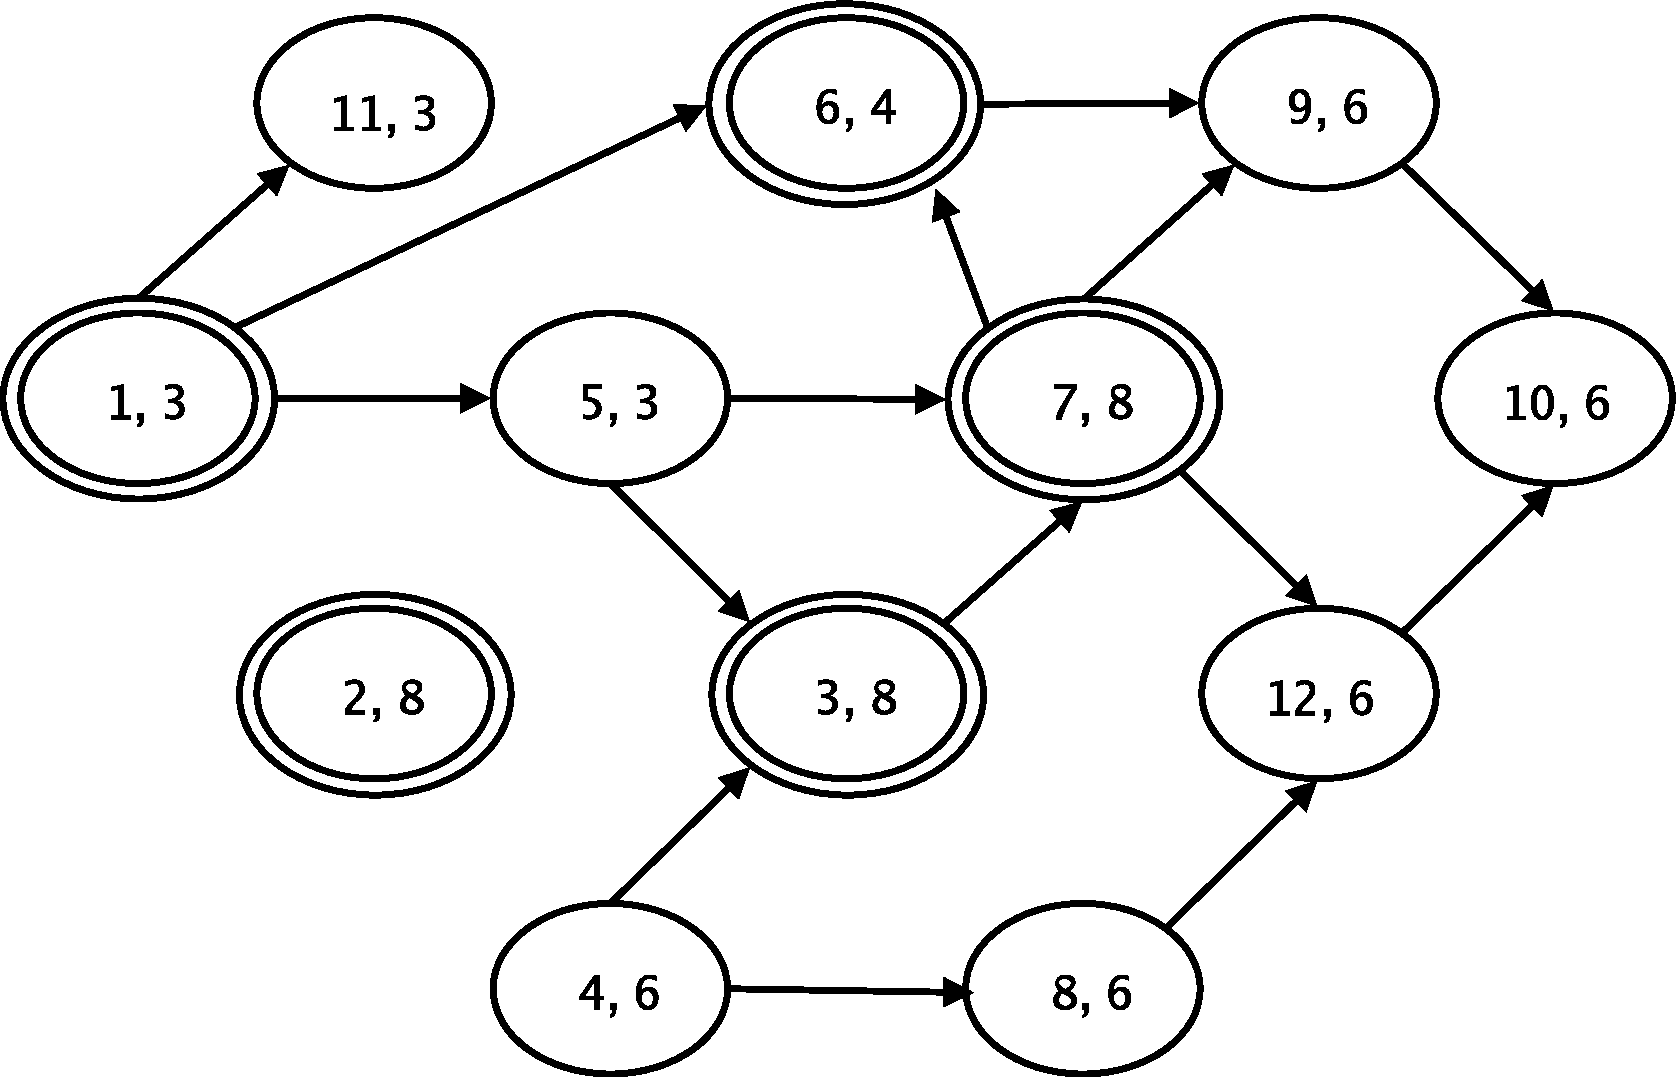
\includegraphics[width=7cm,height=5cm]{opti.pdf}
\caption{Dépendances entre les tâches}
\label{opti}
\end{center}
\end{figure}

This is to find start times for each task, in accordance with these constraints.
\section{Modélisation de la connaissance}
\label{sec:modelisation-connaissance}
We define a symbolic area for machine consists of two
values \verb|m1| and \verb|m2| (This allows the use of
symbolic constraints between variables representing
machines).
It represents a task by a term of the form:

\begin{center}
    \code{tache(Duree, Noms, Machine, Debut)},
\end{center}
where \code{Duree} is an integer giving the duration of the task in minutes
\code{Noms} is a list of clues preliminary tasks in the table
tasks,
 \code{Machine} is the name of the machine and \code{Debut} is a
variable representing the start date.
It represents the data and variables of the problem by an array of such

words:
\begin{center}
\begin{verbatim}
[](tache(3, [],     m1, _),
   tache(8, [],     m1, _),
   tache(8, [4,5],  m1, _),
   tache(6, [],     m2, _),
   tache(3, [1],    m2, _),
   tache(4, [1,7],  m1, _),
   tache(8, [3,5],  m1, _),
   tache(6, [4],    m2, _),
   tache(6, [6,7],  m2, _),
   tache(6, [9,12], m2, _),
   tache(3, [1],    m2, _),
   tache(6, [7,8],  m2, _))
\end{verbatim}
\end{center}

Note that in this problem, the machine that runs each task is known.

\section{Vers une solution en ECLiPSe}
\label{sec:vers-une-solutionOrdo}

\subsection{Une première solution partielle}
\begin{question} \label{TP2_Q1}
Define a predicate \code{taches(?Taches)} that unify \code{Taches} with a task table.
\end{question}

\begin{question}
  Set the iterator that retrieves each element and
   the poster. You will need this type of iterator for
   following questions.
\end{question}


\begin{question} \label{TP2_Q2}
Define a predicate \code{domaines(+Taches, ?Fin)} which requires that any task \code{Taches} starts after time 0 and
finish before the end of (additional variable corresponding to the moment when all tasks are completed).
\end{question}

\begin{question}
Define a predicate \code{getVarList(+Taches, ?Fin, ?List)} which allows to retrieve the list of variables from the problem.
\end{question}

\begin{question}
Define the predicate \code{solve(?Taches, ?Fin)} which uses the previous three predicates to find a schedule that respects the constraints of areas. Check that the solutions given by \eclipse{} are coherent.   
\end{question}

\subsection{Pose des contraintes d'ordonnancement}

NB: For the following two questions, test your
response using simple data.

\begin{question}
Define a predicate \code{precedences(+Taches)} qui contraint chaque tâche à démarrer après la fin de ses
tâches préliminaires. Modifiez \code{solve} pour prendre en compte ces contraintes et vérifiez que les nouvelles solutions proposées par \eclipse{} sont correctes.
\end{question}

\begin{question} \label{TP2_Q4}
Define a predicate\code{conflits(+Taches)} qui impose que, sur une machine, deux tâches ne se déroulent
pas en même temps. Modifiez \code{solve} pour obtenir une solution du problème prenant en compte cette dernière contrainte.
\end{question}

\subsection{La meilleure solution ?}

In this problem, there is a notion of relative quality of
solutions: if a solution $S_1$ is such that the value of
\code{Fin} is less than that of the solution $S_2$, then $S_1$
is better than $S_2$.  We can be interested in the research
the best solution of the problem or the best
solutions.
\begin{question} \label{TP2_last}
 Do you think the solution found by eclipse is the best solution? If so, explain why. Otherwise modify your code to find an optimal solution.
\end{question}


% \section{Optimisation}
% 
% \subsection{Branch and bound dans ic}
% Pour faire de l'optimisation dans le cadre des contraintes à domaine
% finis, le principe de \emph{branch and bound} est généralement
% utilisé. En ECLiPSe, le prédicat \verb|min_max/2| est une
% instanciation de ce principe basée sur la propagation de
% contraintes. Le premier paramètre est un but. Ce but génère un arbre
% de recherche. Le deuxième paramètre est une variable à
% minimiser. \verb|min_max/2| réalise un parcours « intelligent » de
% l'arbre de recherche pour trouver la feuille de l'arbre où la borne
% inférieure du domaine de la variable à minimiser est la plus petite et
% retourne cette borne inférieure. Par conséquent, il faut toujours
% faire un labeling dans le but passé en paramètre de min\_max, sinon la
% valeur rendue peut ne pas correspondre à une solution du problème à
% contraintes. L'exemple suivant
% illustre cette propriété : \verb|[X,Y,Z] :: 1..10, X #= Y+Z, X #= Y*Z|\\
% Utilisez \verb|min_max/2| pour trouver la plus petite valeur de $X$
% solution de ce problème (regardez le manuel d'ECLiPSe pour une
% présentation de min\_max plus approfondie). Essayez sans labeling puis
% avec.
% 
% \begin{question}
% Expliquez les deux valeurs différentes rendues par ECLiPSe.
% \end{question}
% 
% \subsection{Le meilleur ordonnancement}
% \begin{question} \label{TP2_Q6}
% Adresser les requêtes pour trouver un ordonnancement optimal (qui termine au
% plus tôt) et qui respecte les contraintes.
% \end{question}

\section{Compte-rendu}

\subsection{À rendre}

\begin{enumerate}
\item The code \eclipse{} \emph{commenté}. Give eclipse requests
   used to test each question and test data when the data are not the problem.
   For each request, also give the system responses.
\item The detailed answer to the question~\ref{TP2_last} 
\end{enumerate}




% éèàùôê

\chapter{The races}


\section{Problem Statement}
\label{sec:enonce-probleme}


The organizers of a regatta can have 3 yachts each to host a number of teammates. The  accommodation capacities for the yachts are:
\begin{center}
    \begin{tabular}{|c|c|c|}
        \hline
	7&6&5\\
        \hline
    \end{tabular}
\end{center}



4 teams responded to the invitation of the organizers. The size of these
invited teams is given by the following table:

\begin{center}
    \begin{tabular}{|c|c|c|c|}
        \hline
	5&5&2&1\\
        \hline
    \end{tabular}
\end{center}


The puzzle of the organizers then is to try to make a schedule
with the following requirements:

\begin{itemize}

\item The regatta takes place in 3 successive confrontations in which
       3 sailboats compete;

\item invited teams are spread over the 3 boats so
       that :

    \begin{enumerate}

    \item members of the same team stay together,
    \item sailboats of accommodation capacities are met,
    \item during successive confrontations no team returns two time on the same boat,
    \item during successive confrontations no team finds
           with the same partner team.
    \end{enumerate}

\end{itemize}

\clearpage

The goal is to establish a schedule two entries for any confrontation and
for any guest team indicates the number of host sailboat. the schedule
below is a possible answer. It states that during the confrontation 3
Team No. 4 is on the boat 2; it is then Team Partner
2.

\begin{center}
    \begin{tabular}{|c|c|c|c|c|c|c|c|}
        \hline
        \backslashbox{Équipe}{Confrontation} &
         1 &  2 &  3 \\ \hline
         1 &  1 &  2 &  3  \\ \hline
         2 &  3 &  1 &  2  \\ \hline
         3 &  2 &  3 &  1  \\ \hline
         4 &  1 &  3 &  2  \\ \hline
       \end{tabular}
\end{center}


\section{Looking for a solution using ECLiPSe}
\label{sec:vers-une-solutionRegates}

\subsection{A first partial solution}
The problem data are in the form of two vectors: the
vector of terminal facilities and the vector of the sizes of invited teams.
The variables of the problem are the number of \code{NbEquipes * NbConfrontations}. These variables,
representing a host sailboat, have a field \verb|1..NbBateaux|. In the following, the variables are contained in an array with \code{NbEquipes} rows and \code{NbConfrontations} columns.

\begin{question}
 Define the predicate \\\code{getData(?TailleEquipes, ?NbEquipes, ?CapaBateaux, ?NbBateaux, ?NbConf)} \\ that unifies the variables as parameters with the data of problems.
\end{question}


\begin{question}
Define the predicate \code{defineVars(?T, +NbEquipes, +NbConf, +NbBateaux)} which unifies \code{T} the array of variables described above and forced the field variables.
\end{question}

\begin{question}
  Define the predicate \code{getVarList(+T,?L)} which constructs the
  list \code{L} with the variables in the table\code{T}. The variable list must contain the variables of the first column followed by those in the second column, etc. (a test that shows that the order is correct).
  \end{question}

\begin{question}
 Define the predicate  \code{solve(?T)} qui résoud le problème des régates où seules les contraintes de domaines sont posées. 
Vérifiez que les réponses rendues par eclipse vous semblent correctes. 
\end{question}

\subsection{Taking into account problem constraints}

\begin{question}
 Define the predicate\code{pasMemeBateaux(+T, +NbEquipes, +NbConf)}which requires that the same team will not return twice on the same boat.
Modify the predicate \code{solve} to take into account this new constraint and check that the answers given by eclipse are consistent.\end{question}

\begin{question}
 Define the predicate\code{pasMemePartenaires(+T, +NbEquipes, +NbConf)} which requires that the same team is not found twice with the same team.
Modify the predicate \code{solve} to take into account this new constraint and check that the answers given by eclipse are consistent.
\end{question}

\begin{question}
 Define the predicate \\ \code{capaBateaux(+T, +TailleEquipes, +NbEquipes, +CapaBateaux, +NbBateaux, +NbConf)} which verifies that the capacity of ships are met at every confrontation.
Modify the predicate \code{solve} to take into account this new constraint and check that the answers given by eclipse are consistent.\end{question}

\section{let's go ahead with a real-world size problem}

The data used so far are only test data; it would be quite possible to solve the problem without using a computer.
In this section, we consider data more representative of the puzzle that can be organizing a regatta:

We have 13 sailboats whose capacities are listed below:
\begin{center}
    \begin{tabular}{|c|c|c|c|c|c|c|c|c|c|c|c|c|}
        \hline
        10&10&9&8&8&8&8&8&8&7&6&4&4\\
        \hline
    \end{tabular}
\end{center}
  
The number of teams going to 29. The size of each team:
\begin{center}
    \begin{tabular}{|c|c|c|c|c|c|c|c|c|c|c|c|c|c|c|}
        \hline
        7 & 6 & 5 & 5 & 5 & 4 & 4 & 4 & 4 & 4 & 4 & 4 & 4 & 3 & 3\\
        \hline
        \multicolumn{15}{c}{}\\
        \cline{1-14}
        2 & 2 & 2 & 2 & 2 & 2 & 2 & 2 & 2 & 2 & 2 & 2 & 2 & 2 & \multicolumn{1}{c}{}\\
        \cline{1-14}
    \end{tabular}
\end{center}

The regatta takes place in 7 confrontations. First try with
less confrontation and gradually try to 7
confrontations.


Finding a solution to this new problem can be very long! he
you should program your own labeling. Idea to dig:
when you have the list of 29 variables of a confrontation without
doubt it is preferable to get faster a first solution,
reorder the list so as to alternate small and large team.

\begin{question}
 Implement \code{getVarListAlt(+T,?L)} to solve this problem in a reasonable time.
 \end{question}

The following configuration is a solution of the problem:
\begin{center}
    \begin{tabular}{|c|c|c|c|c|c|c|c|}
        \hline
        \backslashbox{Équipe}{Confrontation} &
         1 &  2 &  3 &  4 &  5 &  6 &  7 \\ \hline
         1 &  1 &  2 &  3 &  4 &  5 &  6 &  7 \\ \hline
         2 &  2 &  1 &  4 &  3 &  6 &  5 &  8 \\ \hline
         3 &  3 &  4 &  1 &  2 &  8 &  7 &  9 \\ \hline
         4 &  4 &  3 &  5 &  1 &  2 &  9 & 10 \\ \hline
         5 &  5 &  6 &  2 &  7 &  1 &  3 &  4 \\ \hline
         6 &  6 &  5 &  7 &  2 &  1 &  4 &  3 \\ \hline
         7 &  6 &  7 &  8 &  5 &  2 &  1 & 11 \\ \hline
         8 &  7 &  5 &  6 &  8 &  9 &  1 &  2 \\ \hline
         9 &  8 &  9 &  7 & 10 &  4 & 11 &  5 \\ \hline
        10 &  8 & 10 &  9 &  6 & 11 &  3 &  2 \\ \hline
        11 &  9 &  8 & 12 & 13 &  7 &  2 &  6 \\ \hline
        12 & 10 &  9 &  8 & 11 & 13 & 12 &  1 \\ \hline
        13 & 12 & 13 & 11 &  9 & 10 &  8 &  1 \\ \hline
        14 & 11 & 10 & 13 &  3 &  8 &  9 &  4 \\ \hline
        15 & 11 & 12 & 10 &  7 &  3 & 13 &  9 \\ \hline
        16 & 13 & 11 & 10 &  9 &  6 &  1 &  5 \\ \hline
        17 & 13 &  8 & 11 & 12 &  4 & 10 &  3 \\ \hline
        18 & 10 & 11 &  9 &  8 & 12 &  2 &  3 \\ \hline
        19 &  9 & 11 &  6 & 12 & 10 &  5 & 13 \\ \hline
        20 &  9 &  7 & 10 & 11 & 12 &  8 &  2 \\ \hline
        21 &  7 &  8 &  9 & 10 &  3 &  4 &  1 \\ \hline
        22 &  7 &  6 &  5 &  9 & 11 &  2 &  8 \\ \hline
        23 &  5 &  7 &  1 &  8 &  3 & 10 & 13 \\ \hline
        24 &  4 &  1 &  6 &  5 &  3 &  2 & 12 \\ \hline
        25 &  3 &  2 &  4 &  1 &  7 & 11 & 12 \\ \hline
        26 &  3 &  1 &  2 &  6 &  9 & 10 & 11 \\ \hline
        27 &  2 &  4 &  3 &  1 &  9 &  8 &  6 \\ \hline
        28 &  2 &  3 &  1 &  6 &  7 &  4 &  5 \\ \hline
        29 &  1 &  3 &  2 &  5 &  4 &  7 &  6 \\ \hline
    \end{tabular}
\end{center}
\section{homework}

\subsection{To deliver}

\begin{enumerate}
\item The answer to the problem.
\item The code \eclipse{} \emph{with comments}. Give eclipse requests
   and the system responses.
   \end{enumerate}



\chapter{Constraining thus researching}

\noindent Generally the constraints programs include
two stages, the first is to express the problem and the second
is to find a variable assignment that satisfies
constraints, ie a solution to the problem. We may want
find any solution, all solutions or solution
optimal (or `good 'according to a given criterion). In this problem we
intéresserons the latter type of solution.

%\section{Totalement immoral !}
\section{The problem}
\label{sec:immoral}

Consider the following problem: a production unit can produce
various mobile phone products. The manufacture of the so $ S $
$ N $ mobilizes workers and produces mobile phones $ P $ a day,
for each of these phones benefit is $ E $ euros. The unit has
22 technicians.

It has the following data:

\begin{center}
    \begin{tabular}{|l|r|r|r|r|r|r|r|r|r|}
        \hline
        Sorte & $S_1$ & $S_2$ & $S_3$ & $S_4$ &
                $S_5$ & $S_6$ & $S_7$ & $S_8$ & $S_9$\\ \hline
        Nb. Tech &5&7&2&6&9&3&7&5&3\\ \hline
        Qté jour&140&130&60&95&70&85&100&30&45\\ \hline
        Bénef&4&5&8&5&6&4&7&10&11\\ \hline
    \end{tabular}
\end{center}



We want to know what you have to start manufacturing for the benefit.

\newpage
\section{Model and constrain}

Before coding it is imperative model, that is to say to
the problem equations. To this we must look for a model
general. The problem data are in the form of three
values of vectors: \code{Techniciens}, \code{Quantite},
\code{Benefice}. The variables form a vector\code{Fabriquer}  which
the values will be determined by your program. These values are
either 1 or 0, depending on whether or not the lance production.

\noindent The program must be composed as follows:

\begin{enumerate}
\item part data (facts, variables);
\item part « services predicates (scalar product, \dots);
\item part constraints predicates (equations expressing the problem of properties);
\item part resolution constraints, a predicate that:
    \begin{itemize}
    \item « recovery » data and variables of the problem,
    \item asks the constraints on these variables.
    \end{itemize}
\end{enumerate}

\begin{question} \label{TPCPC_Qdeb} 
  Write predicates that define the three vectors
   values and the vector of variables.
\end{question}

\begin{question}
 Define the predicates which express from
   defined vectors:
\begin{itemize} 
  \item the total number of necessary workers
  \item the vector of total profit by kind of telephone
  \item the total profit
\end{itemize} 
These equations represent predicates using vector operations.
\end{question}

\begin{question}
 Define the predicate: \\
  \code{pose\_contraintes(?Fabriquer, ?NbTechniciensTotal, ?Profit)} which
   poses constraints, then call and list the solutions
   respect these constraints (there are many!).
\end{question}


\section{Optimizing}

\subsection{Branch and bound within ECLiPSe}
To make the optimization under the constraints, the algorithm \emph{branch and bound} is used. 
\newpage
In \eclipse{}, the predicate \code{minimize/2} from the library
\emph{branch\_and\_bound} is an implementation of that algorithm. the
first parameter is a goal. This object generates a search tree which performs
the list of possible solutions. The second parameter is a variable representing the
cost of the solution. It is this variable that should be minimized. 

The predicate \code{minimize / 2} works on the following principle:
as soon as a solution is found, it is stored and research
continues with the additional constraint that the cost is less
than stored. By repeating this process until no longer find
solution, an optimal solution is obtained.

NB: \code {minimize / 2} requires that the object instantiates the variable
cost but not the rest of the variables. In this case, it may
there are no solutions to the problem to obtain the value
optimum found. The following example illustrates this property:
\\\verb|[X,Y,Z,W] #:: [0..10], X #= Z+Y+2*W , X #\= Z+Y+W|

\begin{question}\label{Qmin}
  Use \code{minimize/2} to find the smallest value
   \code{X} solution of this example. Try the labeling only
   \code{X} and finally \code{[X, Y, Z, W]}. Explain the two responses
   made by different \eclipse{}. What must always be in
   the purpose?
\end{question}

\subsection{Application to our problem}

\begin{question}
Call the predicate poses constraints and seek
   "optimal" solution (maximizing profit) and meets the
   constraints posed.
\end{question}

Times change. The mobile market begins to saturate. shareholders
worry. So the company policy fits. We want to produce
less but earn at least 1 \, 000 per day. We want to keep making
mobile lines that ensure this goal but keeping the minimum
workers!

\begin{question} \label{TPCPC_Qfin}
Use the previous approach to address this new problem. There
not much to do (same data, same services predicates, \dots) !
\end{question}

\section{Homework}

\subsection{To do}

\begin{enumerate}
\item The answer to the problem.
\item The commented code. Deliver the queries \eclipse{} and
  the system responses.
\item The detailed answer to the question \ref{Qmin}.
\end{enumerate}



\chapter{Using a swing}
\label{sec:balancoire}


A family of 10 arrived at the park and wants to use a swing
16 seats in the schematic drawing below (seats are spaced
1 meter, except the 2 separate head offices 2 meters)

\begin{center}
    \underline{
      \raisebox{1ex}{\underline{-8 }}
      \raisebox{1ex}{\underline{-7 }}
      \raisebox{1ex}{\underline{-6 }}
      \raisebox{1ex}{\underline{-5 }}
      \raisebox{1ex}{\underline{-4 }}
      \raisebox{1ex}{\underline{-3 }}
      \raisebox{1ex}{\underline{-2 }}
      \raisebox{1ex}{\underline{-1 }}
      ~~~ 
      \raisebox{1ex}{\underline{ 1 }} 
      \raisebox{1ex}{\underline{ 2 }} 
      \raisebox{1ex}{\underline{ 3 }} 
      \raisebox{1ex}{\underline{ 4 }}
      \raisebox{1ex}{\underline{ 5 }} 
      \raisebox{1ex}{\underline{ 6 }} 
      \raisebox{1ex}{\underline{ 7 }}
      \raisebox{1ex}{\underline{ 8 }}
    }

\hspace*{\stretch{1}}\raisebox{2ex}{$\Delta$}\hspace*{\stretch{1}}
\end{center}
The weights of the family members are given in the table below ~:

\begin{center}
    \begin{tabular}{|l|l|l|l|l|l|l|l|l|l|}
        \hline
        24&39 &85 &60 &165 &6  &32 &123 &7  &14 \\
        \hline
        ron&zoe&jim&lou&luc &dan&ted&tom&max&kim\\
        \hline
    \end{tabular}
\end{center}

The constraints of the problem are as follows ~:
\begin{enumerate}
 \item Once installed our 10 people, \textbf{the swing must be balanced} (time left = right time)
 \item Lou and Tom, the mom and dad of the siblings of 8 children, wish
coach their children in order to monitor
 \item Dan and Max, the two
Young people are on two opposite sides, just in front of their mom or dad
 \item there are five persons on each side
\end{enumerate}

\textbf{We are seeking a solution to this problem that minimizes forces moments standards.}

\newpage
Remember: each person $X$ sits down in the swing introduce a force (their weight), note $\overrightarrow{P_X}$. If $d_X$ is the distance between $X$ 
and the swing center, then the norm of the moment exerted on the axis of rotation of the swing by $\overrightarrow{P_X}$ is equal to  $\| \overrightarrow{P_X}\| \times d_X$ 

Here the data of the problem is in the form of a vector of values
: Weight.

The variables (representing places) also form a vector whose $Places$
values will be determined by your program. These values belong to
domain $[-8..-1] \cup [1..8]$. In $Places$ and $Poids$ rank refers implicitly
the person. Although you have to use the vector $Places$ as such, you
will still need to name some variables appear explicitly
in constraints.

\section{Find a solution to the problem}


\noindent The program will be composed as follows :

\begin{enumerate}
\item part data
\item part « services predicates »
\item part defining constraints
\item predicate of calculating a solution using predicates other parts.
\end{enumerate}

Note: as in previous works, it is essential to test code as His. So you-have to start by putting in place predicates That can ask \eclipse{} to find a solution.
When adding an additional constraint, Then you can easily check the impact of this new constraint on the solutions Given by \eclipse{}.

\begin{question}
Write the program that defines the data and sets the constraints of the problem. NB : $ic$ provides various arithmetic constraints that you can use for this lab ($abs/2$, $min/2$, \ldots). Feel free to search the documentation of \eclipse{}!
\end{question}

\begin{question} \label{TP3_Qfin}
Ask \eclipse{} to find a solution.
\end{question}


\begin{question}\label{Qsym}
What symmetry may appear in the solutions to this problem? Remove this symmetry.

What is the impact of this disposal on finding solutions?
\end{question}

\section{Finding the best solution}

\begin{question}
 Use the predicate \code{minimize} from the library \code{branch\_and\_bound} to find the best solution to the problem.
\end{question}

The search for the best solution may be very long, so it is important to help the system to quickly find a good solution. For this, the predicate \code{search / 6} allows you to control the list in two ways:
\begin{itemize}
 \item the order in which the variables are instantiated
 \item the order in which each value of the domain of a variable is tested
\end{itemize}


\begin{version}\label{v1} (see \code{search/6} in the doc)
In this version the first variables considered are those involved in the more constraints (we try to fail as soon as possible to avoid developing unnecessary branches
: « To succeed, try first where you are most likely to fail ! »)
\emph{and} for a given variable values are tried in ascending order.

\emph{If wait too long before finding an optimal solution, interrupt !}
\end{version}


\begin{version}\label{v2} (see \code{search/6} and \code{get\_domain\_as\_list} dans la doc)
In this version the variables are considered in the order of the list, \emph{and} for a given variable values are tested in a sequence suitable to the problem addressed. (In the order of values depends on the order of development of branches when seeking an optimal solution is often an advantage in quickly finding a "good" solution because it will allow a more efficient pruning The order of values depends on. the linear form to be optimized.)

\emph{If wait too long before finding an optimal solution, interrupt !}
\end{version}

\begin{version}
Combine versions \ref{v1} and \ref{v2}.
\end{version}

\begin{version}
Heuristic of choosing the order of the variables calculate a score for each variable according to a specific criterion (see doc \code{search}).
When all variables have the same score, the order in the initial list is used.
Thus, the initial order of the variables can be very important even when using search heuristics.


Submit an initial variable order adapted to the problem and verify the impact of this order on the time to search for the optimal solution.
\end{version}

Note: To reduce the field at the earliest places of Tom and Lou it is possible to state redundant constraints.

\section{Homework}

\subsection{Questions of understanding}

\begin{enumerate}

\item At the end of the year you have been asked to write your own labeling process. What does the original labeling of \eclipse{} and why is it not effective for the problem addressed ~?

\end{enumerate}

\subsection{To deliver}

\begin{enumerate}
\item The answer to the question of understanding.
\item The code \eclipse{}. Give queries \ eclipse {} and the system responses.
\item The answer to the question \ref{Qsym}.
\item A justification of the choices you have made for versions 2 and 4 of the enumeration strategies.
\end{enumerate}



% éèàùôê

\chapter{Les mobiles de Choco}
\label{chapitre:choco}

%%%%%%%%%%%%%%%%%%%%%%%%%%%%%%%%%%%%%%%%%%%%%%%%%%%%%%%%%%%%%%%%%%%%%%%%%%%%%%%%
%                                    TP 5                                      %
%%%%%%%%%%%%%%%%%%%%%%%%%%%%%%%%%%%%%%%%%%%%%%%%%%%%%%%%%%%%%%%%%%%%%%%%%%%%%%%%

\section{Des contraintes sans \prolog{}}

Les problèmes concrets de l'industrie utilisant les contraintes ne sont pas
souvent résolus entièrement en \prolog{}. Il existe alors plusieurs solutions pour
utiliser vos connaissances en programmation par contraintes :

\begin{itemize}

\item utiliser une interface entre \prolog{} et le langage utilisé dans le reste
      du projet (par exemple ECLiPSe s'interface très bien avec JAVA et C++)~;

\item utiliser un autre moteur de résolution des contraintes (i.e. un autre
      solveur) dans un autre langage. 

\end{itemize}

C'est cette dernière solution que nous allons explorer dans ce chapitre. Il
existe beaucoup de moteurs dans différents langages, pour n'en citer que
quelques uns :

\begin{itemize}
	\item en C++ : Disolver, gecode, \ldots
	\item en Java : JaCob, JCK, JCL, Choco, \ldots
	\item en Ocaml : FaCiLe, \ldots
\end{itemize}

Nous allons utiliser \textbf{Choco} pour résoudre un problème simple dans le
domaine des entiers dans un programme Java. Vous trouverez en annexe
\ref{annexe:choco} un descriptif des fonctionnalités de Choco pour poser et
résoudre les problèmes. Vous pouvez aussi aller voir sur le site de Choco
\url{http://www.emn.fr/z-info/choco-solver/index.html}. 

Nous vous fournissons une grosse partie du code Java, il ne reste que
la partie programmation des contraintes à réaliser. Ce code est fourni
à l'emplacement \url{/home-info/commun/4info/Contraintes_choco} de
votre machine.

\section{Le problème : équilibrer un mobile}

Le problème que nous considérons est l'équilibrage d'un mobile de structure
fixée décrite par la figure \ref{fig:mobile} (il n'est pas demandé de résoudre
le problème dans le cas général, même si la programmation objet de Java le
permettrait facilement).

\begin{figure}
\begin{center}
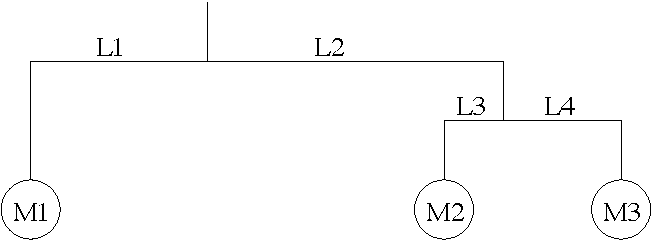
\includegraphics[width=10cm]{mobile.pdf}
\caption{Le mobile à équilibrer}
\label{fig:mobile}
\end{center}
\end{figure}

Le problème comporte donc 7 variables entières (problème dans le domaine fini) :

\begin{itemize}

\item les longueurs des branches : L1 et L2 pour le premier étage et L3 et L4
      pour le second ;

\item les masses M1, M2 et M3 au bout des branches.

\end{itemize}

Le mobile est soumis à quelques contraintes (physiques). Le mobile doit pouvoir
tourner (une contrainte entre les longueurs à valeurs entières) sachant que les
masses sont de tailles négligeables. Le mobile doit être équilibré (ce qui
correspond à deux contraintes entre les variables). Pour équilibrer le mobile
on dispose de 20 masses différentes, dont les poids à valeur entière
s'échantillonnent de 1 à 20g.

\section{Les problèmes à résoudre}

\begin{question}
Écrire les programmes qui résolvent les deux problèmes qui suivent.
\end{question}

\begin{enumerate}
\item L'utilisateur entre des valeurs pour les longueurs des branches, vous
      devez vérifier que ces longueurs sont cohérentes ;

\item Trouver les masses M1, M2 et M3 qu'il faut choisir parmi les poids
      disponibles pour équilibrer les mobiles (ce qui n'est pas toujours
      possible mais parfois il existe plusieurs solutions).

\end{enumerate}

Il faut définir les variables et leurs domaines puis poser les différentes
contraintes. Il vous sera indiqué en TP quelles méthodes Java compléter.


% éèàùôê

\chapter{Histoire de menteurs}

%%%%%%%%%%%%%%%%%%%%%%%%%%%%%%%%%%%%%%%%%%%%%%%%%%%%%%%%%%%%%%%%%%%%%%%%%%%%%%%%
%                                    TP 4                                      %
%%%%%%%%%%%%%%%%%%%%%%%%%%%%%%%%%%%%%%%%%%%%%%%%%%%%%%%%%%%%%%%%%%%%%%%%%%%%%%%%


\setlength{\parskip}{2ex}
\setlength{\parindent}{0pt}

\section{Le puzzle}
\label{sec:mensonge}

Parent1 et Parent2 forment un couple hétérosexuel, mais on ne sait pas qui est la femme ni
qui est l'homme ! Ces deux personnes ont un enfant Enfant dont on ne connaît pas le
sexe.

Le seul critère permettant de discerner femmes et hommes est le suivant :

\begin{enumerate}
\item Les femmes disent toujours la vérité.
\item Les hommes alternent systématiquement vérité et mensonge.
\end{enumerate}

(Selon vos convictions, vous pouvez bien sûr adapter l'énoncé \ldots)

On demande à Enfant s'il est un homme ou une femme :

\begin{tabbing}
  \hspace{2.5em} Enfant affirme : Arrheu, arrheu~!
\end{tabbing}
On se tourne alors vers ses parents Parent1 et Parent2.
\begin{tabbing}
  \hspace{2.5em}\= Parent1 affirme : Enfant vous dit qu'elle est une femme.\\
                \> Parent2 affirme : Enfant est un homme puis \dots\\
                \> Parent2 affirme : Enfant ment.
\end{tabbing}

On cherche à savoir qui est le père, qui est la mère et quel est le sexe de l'enfant.


\section{Modélisation}

Modéliser ce puzzle logique en utilisant les contraintes logiques de la
bibliothèque \emph{ic}. Pour cela, identifier les variables et leur domaine.

\begin{question}
« Les femmes disent toujours la vérité. ». \\
Définir le prédicat \code{affirme/2} tel que \code{affirme(?S,?A)} pose
la contrainte : l'affirmation \code{A} est vraie si \code{S} est une
femme.
\end{question}

\begin{question}
« Les hommes alternent systématiquement vérité et mensonge. » \\
Définir le prédicat \code{affirme/3} tel que \code{affirme(?S,?A1,?A2)}
pose la contrainte~: si \code{S} est un homme, les affirmations $A_1$
et $A_2$ sont l'une vraie, l'autre fausse.
\end{question}
\begin{tabbing}
  \hspace{2.5em}\= AffE  est l'affirmation de l'enfant.\\
                \> AffEselonP1 est l'affirmation de l'enfant selon Parent1.\\
                \> AffP1 est l'affirmation de Parent1.\\
                \> Aff1P2 est la première affirmation de Parent2.\\ 
                \> Aff2P2 est la seconde affirmation de Parent2.
\end{tabbing}

Chacune de ces affirmations appartient au domaine booléen $\{0,1\}$ (représenté par l'intervalle entier [0..1]) :
\begin{tabbing}
  \hspace{2.5em}\= AffEselonP1 : \hspace{1em}\= Enfant est une femme\\
                \> AffP1       :             \> AffEselonP1 = AffE\\
                \> Aff1P2      :             \> Enfant est un homme\\
                \> Aff2P2      :             \> AffE = 0
\end{tabbing}

\begin{question}
  Définir le domaine symbolique des variables \code{Parent1}, \code{Parent2} et \code{Enfant}, puis écrire le prédicat qui contraint
  le domaine de l'ensemble des variables.  
\end{question}

\begin{question} 
  Poser les contraintes sur les variables et définir un prédicat de labeling pour les valeurs symboliques (comme pour le TP \ref{tp2}). Utilisez ce prédicat pour résoudre le problème.
\end{question}

% \section{Compte-rendu}

% \subsection{À rendre}

% \begin{enumerate}
% \item La réponse au problème posé.
% \item Le code \eclipse{} \emph{commenté}. Donnez les requêtes ainsi que les réponses du système. 
% \end{enumerate}





%%%%%%%%%%%%%%%%%%%%%%%%%%%%%%%%%%%%%%%%%%%%%%%%%%%%%%%%%%%%%%%%%%%%%%%%%%%%%%%%
%                                   Annexes                                    %
%%%%%%%%%%%%%%%%%%%%%%%%%%%%%%%%%%%%%%%%%%%%%%%%%%%%%%%%%%%%%%%%%%%%%%%%%%%%%%%%

\appendix

\chapter{Utilisation du solveur Choco}
\label{annexe:choco}

Cette annexe présente les éléments utiles pour réaliser le TP sur les mobiles
avec le solveur Choco, écrit en Java. Pour plus de renseignements, se référer
au site:\\
\centerline{\url{http://www.emn.fr/z-info/choco-solver/index.html}}

%%NB : Afin de simplifier la prise en main rapide du solveur, certaines signatures de méthodes ont été modifiées par rapport à la documentation du solveur pour n'accepter que certains sous-types intéressants pour le TP.

\subsection*{Faire appel à la bibliothèque Choco}

La bibliothèque Choco est disponible sous forme de .jar. Sous l'environnement
de développement pour Java ECLiPSe, il suffit d'inclure le chemin vers la
bibliothèque dans le classpath du projet (menu Project, Properties, Java Build
Path, onglet Libraries, bouton Add External JARs \ldots).\\
Il faut importer en tête de fichier les classes de Choco qui seront utilisées.
Dans notre cas:\\
\texttt{import static choco.Choco.*;}
%%\texttt{import choco.integer.IntDomainVar;}

\subsection*{Architecture générale choco}
On identifie clairement deux parties différentes sur le schéma \ref{choco}:
\begin{enumerate}
\item modélisation du problème via la classe Model
%%\begin{itemize}
%%\item variables
%%\item contraintes
%%\end{itemize}
\item résolution du problème via la classe Solver
\end{enumerate}

\begin{figure}[!ht]
\begin{center}
%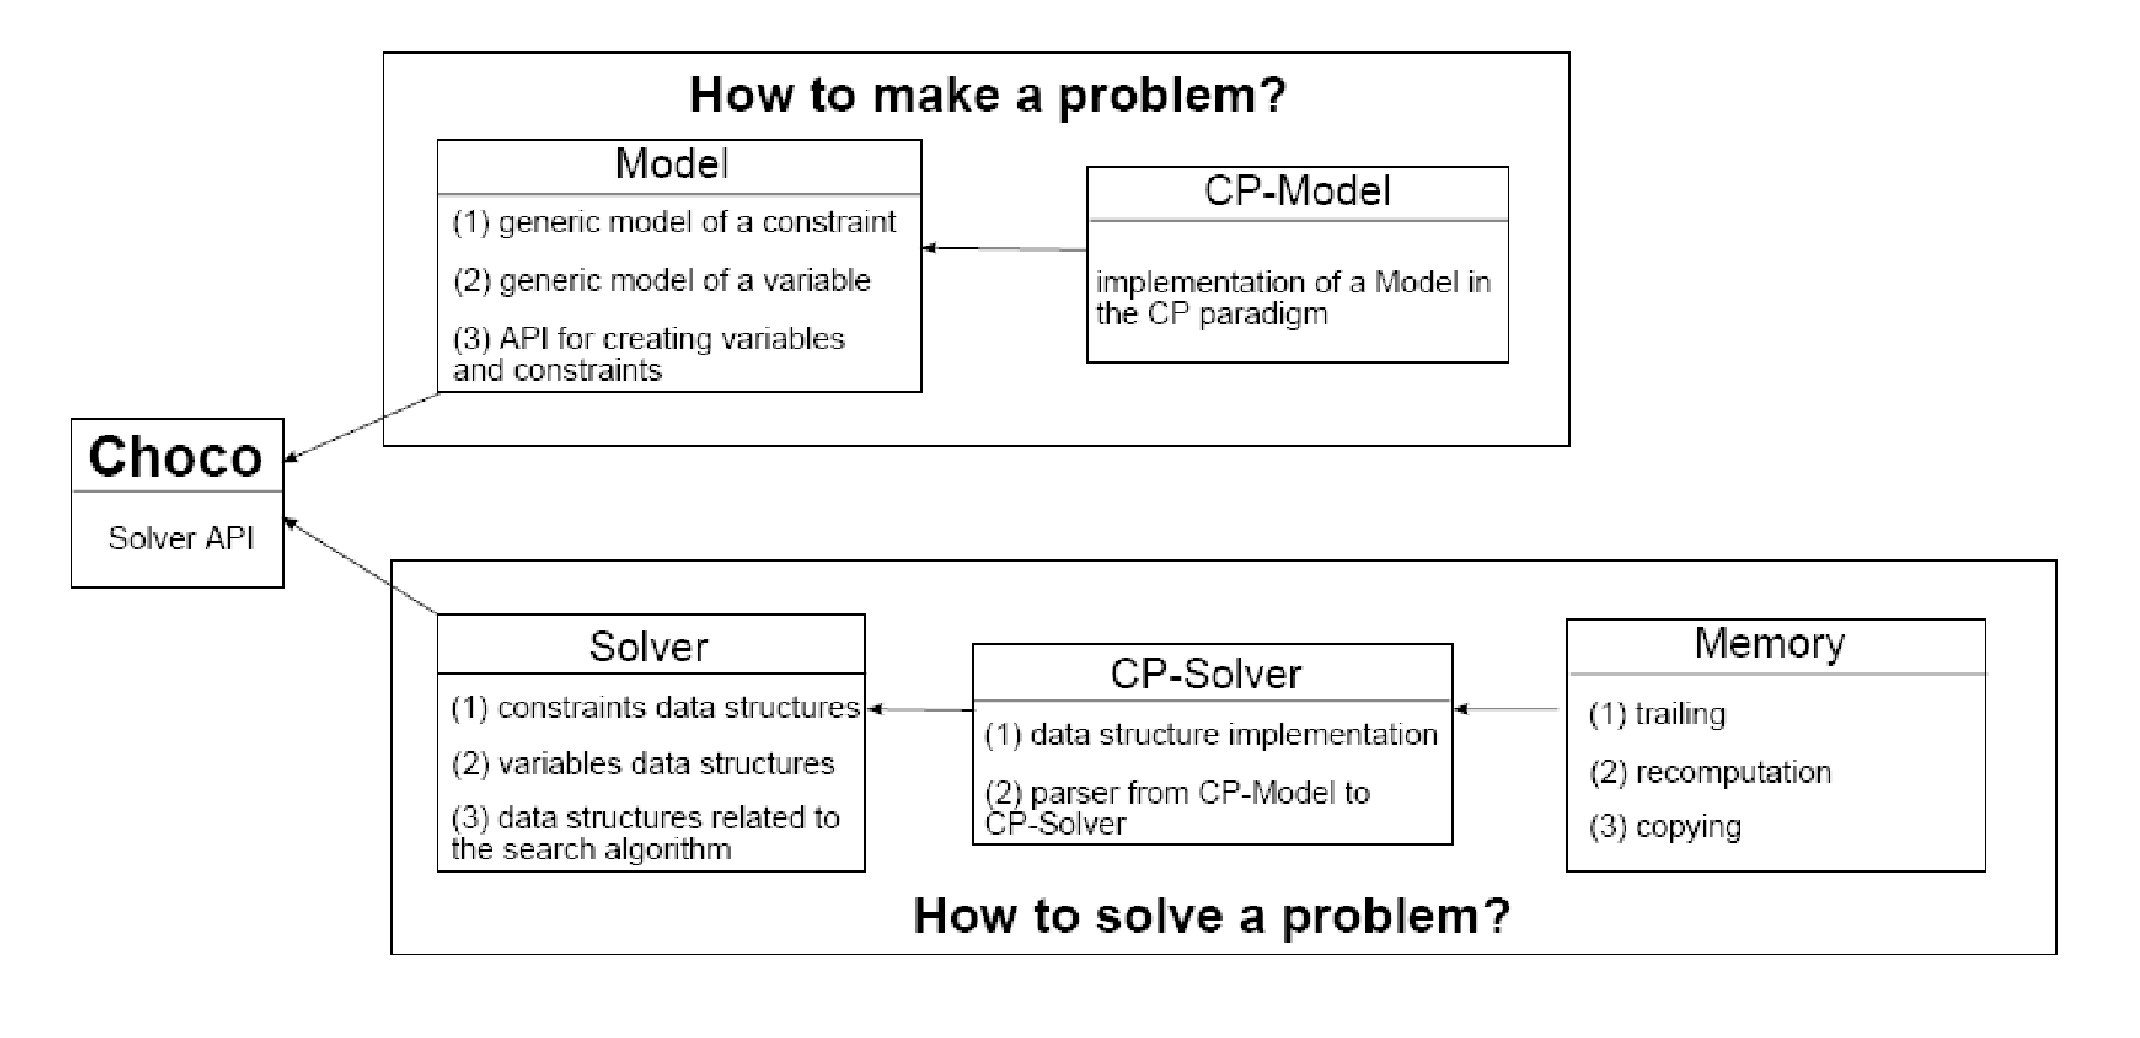
\includegraphics[width=16cm,height=6cm]{choco.pdf}
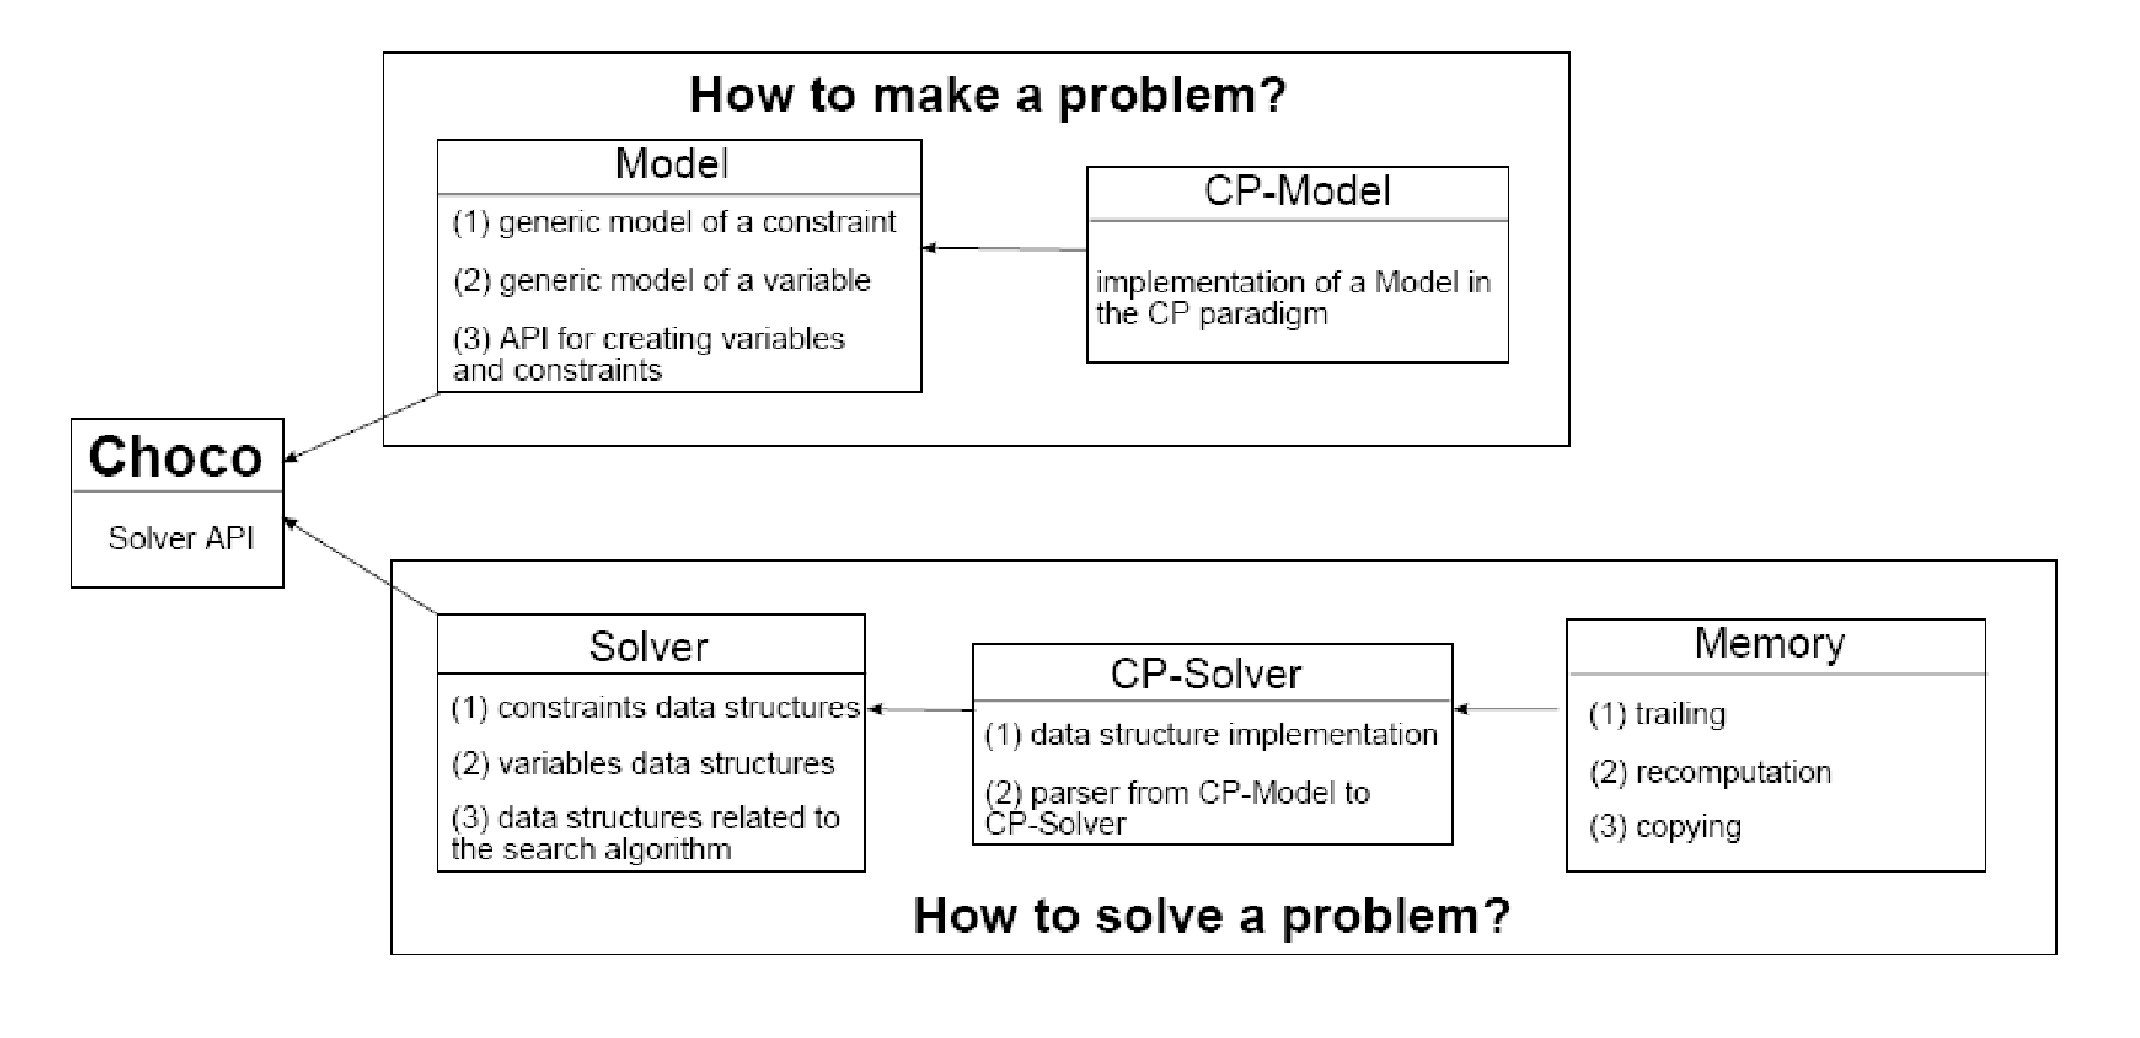
\includegraphics[width=\linewidth]{choco.pdf}
\caption{Architecture choco}
\label{choco}
\end{center}
\end{figure}
Détaillons ces étapes.


\subsection*{Modéliser un problème}
En Choco, le problème à résoudre par programmation par contraintes est une instance de la classe \texttt{Model}.\\
Constructeur d'un objet de type \texttt{Model} : \texttt{CPModel()}

\`A un objet de type \texttt{Model}, on associe:
\begin{enumerate}

\item des variables. Dans notre cas, il s'agit de variables entières à domaine
      fini.

  \begin{itemize}

  \item Déclaration:\\
  \hspace{0.5 cm} \texttt{IntegerVariable makeIntVar(String nom,int borne\_min,int borne\_max)}\\
     où \texttt{nom} est le nom de la variable, \texttt{borne\_min} et
     \texttt{borne\_max} sont les bornes inférieure et supérieure de son domaine
     de définition.

  \item Association à l'objet \texttt{Model}:\\
  \hspace{0.5 cm} \texttt{void Model$\colon\colon$addVariable(IntegerVariable var);}
  \end{itemize}

  \item des contraintes.

  \begin{itemize}
  \item Déclaration: on dispose d'un large panel de contraintes. Les plus
        utiles sont listées dans le paragraphe ci-dessous.

  \item Association à un objet \texttt{Model}:

  \hspace{0.5 cm} \texttt{void Model$\colon\colon$addConstraint(Constraint c);}
  \end{itemize}

\end{enumerate}

Imports en tête de fichier : \texttt{import choco.cp.model.CPModel;}\\
\texttt{import choco.kernel.model.variables.integer.IntegerVariable;}

\subsection*{Exprimer une contrainte}

Les contraintes sont exprimées sur des instances de la classe
\texttt{IntegerExpressionVariable}. Cette classe permet de représenter des
expressions linéaires entières (nous le notons par la suite IEV pour des
raisons de lisibilité). La classe représentant les variables sur les domaines
finis est \texttt{IntegerVariable}, elle hérite de
\texttt{IntegerExpressionVariable}.

\noindent Opération d'addition et de multiplication :\\
\texttt{IEV plus(IEV t1, IEV t2)}\\
\texttt{IEV mult(int i, IEV t)}

\noindent Contrainte d'égalité :\\
\texttt{Constraint eq(IEV t1, IEV t2)}

\noindent Contrainte de stricte infériorité :\\
\texttt{Constraint lt(IEV t1, IEV t2)}

\noindent Contrainte allDifferent :\\
\texttt{Constraint allDifferent(IV[] tab)}\\
\indent où \texttt{tab} contient les variables dont on veut contraindre les
        valeurs à être toutes différentes

\subsection*{Résoudre un problème}

Afin de résoudre un problème, on va déclarer un solveur, instance de la classe
\texttt{Solver}, et l'associer au modèle.

Constructeur d'un objet de type \texttt{Solver} :\\
\texttt{CPSolver()}

Lecture du modèle par le solveur:\\
\texttt{void Solver$\colon\colon$read(Model model)}

Lancer la résolution du système de contraintes :\\
\texttt{java.lang.Boolean Solver$\colon\colon$solve()}\\
\indent rend vrai si une solution est trouvée. Les variables sous contraintes
        sont instanciées avec les valeurs formant cette solution.

Trouver une nouvelle solution :\\
\texttt{java.lang.Boolean Solver$\colon\colon$nextSolution()}\\
\indent rend vrai si une nouvelle solution est trouvée.

Il n'est pas possible d'accéder à la valeur ou au domaine d'une variable
lorsque le processus de résolution a été appliqué par l'intermédiaire du
modèle (l'instance \texttt{Model}). Il faut pour cela utiliser le solveur.

Récupérer le domaine de la variable :\\
\texttt{IntDomainVar Solver$\colon\colon$getVar(IEV var)}

Accéder à la valeur si instanciée (valeur pour la solution courante):\\
\texttt{int IntDomainVar$\colon\colon$getVal()}

Import en tête de fichier :\\
\texttt{import choco.cp.solver.CPSolver;}


\end{document}
